%%%%%%%%%%%%%%%%%%%%%%%%%%%%%%%%%%%%%%%%%%%%%%%%%%%%
\graphicspath{{}{dark_nus/}{Diagrams/}}

The most important evidences that the Standard Model (SM) of particle physics is incomplete are neutrino masses and mixing, and the presence of dark matter (DM) in the Universe. Both call for extensions of the SM and the possible existence of dark sectors which do not partake in SM interactions, or do so with extremely weak couplings while displaying strong ``dark" interactions~\cite{Boehm:2003hm,Boehm:2003ha,Alexander:2016aln}.
Such sectors might exist at relatively light scales below the electroweak one, being within reach of present and future non-collider experiments. Generically, a neutral dark sector can communicate with the SM via three renormalizable portals. New neutral fermions mix with light neutrinos unless a symmetry differentiates the two, a possibility usually denoted as the neutrino portal. New vector particles can kinetically mix with the SM hypercharge, and new scalars mix with the Higgs boson through the so-called vector and scalar portals, respectively. The latter terms are generically allowed in the Lagrangian and an explanation of their smallness requires specific UV completions.  

In this article, we propose a new neutrino model with a hidden $U(1)^\prime$ gauge symmetry under which no SM fields are charged. We introduce new SM-neutral fermions, $\nu_D$ and an additional sterile neutrino $N$. The symmetry is subsequently broken by the vacuum expectation value (vev) of a complex dark scalar $\Phi$, which gives mass to the new gauge boson. For concreteness, we restrict the scale of the breaking to be below the electroweak one. 

Models with heavy neutrinos which are not completely sterile and might participate in new gauge interactions have been studied in several contexts, including $B-L$, $L_\mu-L_\tau$ and left-right symmetric models~\cite{%
Buchmuller:1991ce,% original
Khalil:2006yi,% B-L at TeV scale
Perez:2009mu,% B-L extensive discussion + X model
Khalil:2010iu,% B-L at collider and ISS
Dib:2014fua,% B-L in linear seesaw
Baek:2015mna,% mu-tau in inverse seesaw
DeRomeri:2017oxa,% Elusive B-L
Nomura:2018mwr,% U(1)_R
Brdar:2018sbk% LR symmetry low scale
}, but here we focus on the possibility of a symmetry under which no SM fields are charged~\cite{%
Okada:2014nsa,% U(1)prime
Diaz:2017edh,% Hidden with loops
Nomura:2018ibs% Hidden in linear seesaw
}. New heavy neutral fermions that feel such hidden forces, such as $\nu_D$, are referred to as \textit{dark neutrinos}, since they define a dark sector separate from the SM. Nevertheless, the dark interactions ``leak" into the SM sector via neutrino mixing, where they may dominate~\cite{Pospelov:2011ha,Batell:2016zod}. Models of this type have been invoked to generate large neutrino non-standard interactions~\cite{Farzan:2015doa,Farzan:2016wym}, generate new signals in DM experiments~\cite{Pospelov:2011ha,Pospelov:2012gm,Pospelov:2013rha,Harnik:2012ni,McKeen:2018pbb}, weaken cosmological and terrestrial bounds on eV scale sterile neutrinos~\cite{Hannestad:2013ana,Dasgupta:2013zpn,Mirizzi:2014ama,Chu:2015ipa,Cherry:2016jol,Chu:2018gxk,Denton:2018dqq,Esmaili:2018qzu}, and as a potential explanation of anomalous short-baseline results at the MiniBooNE~\cite{AguilarArevalo:2007it,Aguilar-Arevalo:2018gpe} and/or LSND~\cite{PhysRevLett.77.3082,Aguilar:2001ty} experiments with new degrees of freedom at the MeV/GeV scale~\cite{Gninenko:2009ks,Gninenko:2010pr,Masip:2012ke,Radionov:2013mca,Ballett:2018ynz,Bertuzzo:2018itn,Arguelles:2018mtc}.

Our model presents all the three renormalizable portals to the SM. The Yukawa interactions between the leptonic doublet and $N$, and between $N$ and $\nu_D$ induce neutrino mixing. 
The gauge symmetry allows a cross-coupling term in the potential between the Higgs and the real part of the scalar, inducing mixing between the two after symmetry breaking. The broken gauge symmetry implies the existence of a light hidden gauge boson $X_\mu$, which mediates the dark neutrino interactions and generically kinetically mixes with the SM hypercharge. The set-up is self-consistent and combines the three portals into a unified picture that exhibits significantly different phenomenology with respect to each portal taken separately, as we discuss. The interplay of the different portal degrees of freedom leads to novel signatures which would have escaped searches performed to date, and that can explain long-standing anomalies. For the latter, we focus on the MiniBooNE anomaly as discussed in Ref.~\cite{Ballett:2018ynz} (see also~\cite{Bertuzzo:2018itn}) and on new neutrino scattering signatures at neutrino experiments~\cite{Arguelles:2018mtc}. We also reconsider the possibility to explain the discrepancy between the prediction and measurement of the anomalous magnetic moment of the muon ($\Delta a_\mu$)~\cite{Bennett:2006fi} via kinetic mixing~\cite{Fayet:2007ua,Pospelov:2008zw}.

An interesting feature of the model is the generation of neutrino masses at loop-level. This requires only two key features of our setup, namely a light $Z^\prime$ and neutrino mixing, but not the vector and scalar portals. For this reason, we discuss it elsewhere~\cite{Ballett:2019cqp}.

In its minimal form, the model is not anomaly-free. We discuss how this can be cured and propose a minor extension that introduces additional dark sector neutral fermions charged under the new symmetry~\cite{Boehm:2003hm,Boehm:2003ha}. Neutrinos, we argue, may be a window into such dark sectors, bridging the puzzles of neutrino masses and DM~\cite{Ma:2006km,Farzan:2009ji,Farzan:2010mr,Arhrib:2015dez,Cherry:2014xra,Escudero:2016tzx,Escudero:2016ksa,Batell:2017cmf,Capozzi:2017auw,Campo:2017nwh,Blennow:2019fhy}. We briefly outline the key features of a DM extension and leave a more detailed analysis to future work.

%%%%%%%%%%%%%%%%%%%%%%%%%%%%%%
%
\begin{figure}[t]
\centering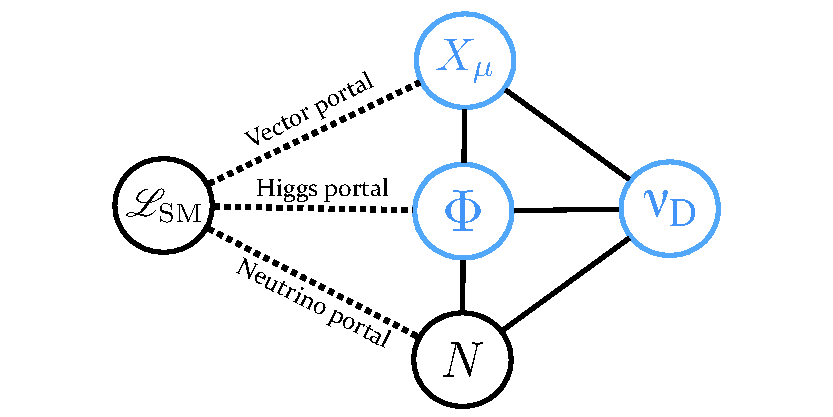
\includegraphics[width=0.7\textwidth]{portals.pdf}
\caption[Dark neutrino model diagram.]{Schematic representation of our dark neutrino model. The dark neutrino, $\nu_{D}$ and the complex scalar $\Phi$ are the only fields charged under the new U$(1)^\prime$ gauge symmetry. The new vector boson $X_\mu$ acquires a mass after spontaneous symmetry breakig, and $N$ remains a complete singlet.
\label{fig:Tdiagrams}}
\end{figure}
%
%%%%%%%%%%%%%%%%%%%%%%%%%%%%%%



%%%%%%%%%%%%%%%%%%%%%%%%%%%%%%%%%%%%%%%%%%%%%%%%%%%%%%%%%%%%%%%%%%%%%%%
\section{The Model} 
We extend the SM gauge group with a new abelian gauge symmetry $U(1)^\prime$ with associated mediator $X_\mu$ and introduce three new singlets of the SM gauge group: a complex scalar $\Phi$, and two left-handed fermions $\nu_{D,L} \equiv \nu_{D}$ and $N_L \equiv N$. 
%As shown in \reftab{tab:fields}, t
The scalar $\Phi$ and the fermion $\nu_{D}$ are equally charged under the new symmetry, and $N$ is neutral with respect to all gauge symmetries of the model. For simplicity, we restrict our discussion to a single generation of hidden fermions. The relevant terms in the gauge-invariant Lagrangian are 
%
\begin{align} \label{eq:lagrangian}
%
\mathscr{L}  \supset  &\left(D_\mu \Phi\right)^\dagger \left(D^\mu \Phi\right) -  V(\Phi,H) \,   \nonumber\\
&  - \frac{1}{4}X^{\mu \nu} X_{\mu \nu} + \overline{N}i\slashed{\partial}N + \overline{\nu_D}i\slashed{D}\nu_D 
\nonumber\\
&- \left[y^\alpha_\nu (\overline{L_\alpha} \cdot \widetilde{H})N^c + \frac{\mu^\prime}{2}\overline{N}N^c + y_N \overline{N}\nu_D^c\Phi + \text{h.c.}\right],
\end{align}
%
where $X^{\mu\nu}$ is the field strength tensor for $X_{\mu}$, $D_\mu \equiv \left(\partial_\mu-ig^\prime X_\mu\right)$ the covariant derivative, $L_\alpha \equiv (\nu_\alpha^T, \ell_\alpha^T)^T$ the SM leptonic doublet of flavour $\alpha = e, \mu, \tau$ and $\widetilde{H} \equiv i \sigma_2 H^*$ is the charge conjugate of the SM Higgs doublet. We write $y_\nu^\alpha$ for the $L_\alpha$--$N$ Yukawa coupling, $y_N$ for the $\nu_D$--$N$ one, and $\mu^\prime$ for the Majorana mass of $N$, which is allowed by the SM and the new gauge interaction, although it breaks lepton number by 2 units.

The minimisation of the scalar potential $V(\Phi,H)$ leads the neutral component of the fields $H$ and $\Phi$ to acquire vevs $v_H$ and $v_\varphi$, respectively. The latter also generates a mass for both the new gauge boson $X_\mu$ and the real component of the scalar field $\varphi$. Although $v_\varphi$ is arbitrary, we choose it to be below the electroweak scale, $v_\varphi < v_H$, as we are interested in building a model testable at low scales.

\paragraph{Neutrino portal}
In the neutral fermion sector and after symmetry breaking, two Dirac mass terms are induced with $m_D \equiv y_\nu^\alpha v_H/\sqrt{2}$ and $\Lambda \equiv y_N v_\varphi/\sqrt{2}$.
It is useful to consider the form of the neutrino mass matrix in the single generation case to clarify its main features. For one active neutrino $\nu_\alpha$ ($\alpha= e, \mu, \tau$), it reads
%
\begin{align} \label{eq:massmatrix}
\mathscr{L}_{\rm mass} \supset
\frac{1}{2}\left (\begin{matrix} \overline{\nu}_\alpha & \overline{N} &  \overline{\nu_D} \end{matrix} \right )
\left(\begin{matrix} 
     0   &  m_D        & 0 
\\ m_D &  \mu^\prime & \Lambda 
\\   0   &  \Lambda  & 0
\end{matrix}\right)
\left (\begin{matrix} \nu_\alpha^c \\ N^c \\ \nu_D^c \end{matrix} \right) + {\rm h.c.}
\end{align}  
%
The form of this matrix appears in Inverse Seesaw (ISS)~\cite{Mohapatra:1986bd,GonzalezGarcia:1988rw} and in Extended Seesaw (ESS)~\cite{Barry:2011wb,Zhang:2011vh} models. In fact, it is the same matrix discussed in the so-called Minimal ISS~\cite{Dev:2012sg}, with the difference that in our case its structure is a consequence of the hidden symmetry.
After diagonalisation of the mass matrix, the two heavy neutrinos, $\nu_h$ with $h=4,5$, acquire masses. Assuming that $m_D \ll \Lambda$, we focus on two interesting limiting cases. 

In the \textit{ISS-like} limit, where $\Lambda \gg \mu^\prime$ and the two heavy neutrinos are nearly degenerate, we have 
\begin{align}
 m_5 \simeq - m_4 \simeq \Lambda ~,  \,\,  m_5-|m_4| = \mu^\prime ~,& \nonumber\,\,
 U_{\alpha 5} \simeq U_{\alpha 4} \simeq  \frac{m_D}{\sqrt{2}\Lambda}~, \\   U_{D i} \simeq \frac{m_D}{\Lambda}, \,\, U_{D5} \simeq U_{D4} \simeq \frac{1}{\sqrt{2}} ~, \,\, & U_{N5} \simeq U_{N4} \simeq \frac{1}{\sqrt{2}} ~.\nonumber
\end{align}

In the \textit{ESS-like} case, $\Lambda \ll \mu^\prime$, one neutral lepton remains very heavy and mainly in the completely neutral direction $N$, and the other acquires a small mass via the seesaw mechanism in the hidden sector. We find
%
\begin{align}
m_4 \simeq -\frac{ \Lambda^2}{\mu^\prime}~, & \,\,  m_5 \simeq \mu^\prime ~, \,\, U_{\alpha 4} \simeq U_{\alpha 5}\sqrt{\frac{m_5}{\left|m_4\right|}}  \simeq  \frac{m_D}{\Lambda}~,\nonumber \\ \,\, U_{D i} \simeq \frac{m_D}{\Lambda},  &\,\,  U_{N5} \simeq U_{D4} \simeq 1 ~, \,\,  U_{D5} \simeq U_{N4} \simeq \frac{\Lambda}{\mu^\prime} ~.\nonumber
\end{align}
%
From the discussion above, it is clear that the masses of $Z^\prime$ and $\varphi^\prime$ are typically above the heavy neutrino ones, unless we are in the ESS-like regime.

The Yukawa terms in \refeq{eq:lagrangian} induce {\em neutrino mixing} between the active (light) and heavy (sterile, dark) neutrinos. In this model, similarly to the ISS and the ESS cases, this mixing can be much larger than the typical values required in type-I seesaw extensions to explain neutrino masses, making its phenomenology more interesting. The determinant of the mass matrix in \refeq{eq:massmatrix} is zero, and so light neutrino masses vanish at tree-level and do not constrain the values of the active-heavy mixing angles. This, however, is no longer the case at one-loop level, as light neutrino masses emerge through radiative corrections from diagrams involving the $\varphi^\prime$ and $Z^\prime$ degrees of freedom~\cite{Ballett:2019cqp}.  


\paragraph{Scalar portal}
In the scalar potential, the symmetries of the model allow us to write down the following term
\begin{equation}
    V(\Phi,H) \supset \lambda_{\Phi H} \, H^\dagger H \left| \Phi\right|^2,
\end{equation}
where we identify $\lambda_{\Phi H}$ as the scalar portal coupling~\cite{Barger:2008jx}, responsible for mixing in the neutral scalar sector. If such a term exists, the scalar mass eigenstates $(h^\prime, \varphi^\prime)$ mix with the gauge eigenstates $(h, \varphi)$ 
%as $h^\prime = h \cos{\alpha}  - \varphi \sin{\alpha} $ and  $\varphi^\prime = h \sin{\alpha}  + \varphi \cos{\alpha}$,
with a mixing angle $\alpha$ defined by 
%
\begin{equation}
\tan{(2\alpha)} \equiv \frac{\lambda_{\Phi H} v_{H} v_\varphi}{\lambda_h v_{H}^2 - \lambda_\varphi v_\varphi^2},
\end{equation}
%
where $\lambda_h$ and $\lambda_\varphi$ are the quartic couplings of the Higgs and $\Phi$ scalars, respectively. 

\paragraph{Vector portal}  Similarly, mixing also arises in the neutral vector boson sector from the allowed kinetic mixing term~\cite{Holdom:1985ag}
%
\begin{equation}
 \mathscr{L} \supset - \frac{\sin{\chi}}{2} \, F^{\mu \nu} X_{\mu \nu},
\end{equation} 
%
where $F_{\mu\nu}$ is the SM hypercharge field strength. This term may be removed with a field redefinition, resulting in three mass eigenstates $\left( A,\, Z^0,\, Z^\prime\right)$, corresponding to the photon, $Z^0$-boson and the hypothetical $Z^\prime$-boson. For a light $Z^\prime$, the $Z^\prime$ coupling to SM fermions $f$ to first order in the small parameter $\chi$ is given by
%
\begin{equation}
\mathscr{L} \supset - (e\,q_f\,c_{W}) \chi \,\overline{f} \gamma^\mu f\,Z^\prime_\mu ~,
\end{equation}
%
with  $q_f$ the fermion electric charge.

The values of $\chi$ and $\lambda_{\Phi H}$ are arbitrary and could be expected to be rather large. As such, we treat them as free parameters within their allowed ranges. Here, we merely note that with our current minimal matter content, $\chi$ and $\lambda_{\Phi H}$ receive contributions at loop level from the $(\overline{L}_\alpha \cdot \widetilde{H})N^c$ and $\overline{N} \nu_D^c \Phi$ terms, which are necessarily suppressed by neutrino mixing ($\chi \propto g^\prime e |U_{\alpha h}|^2$ and $\lambda_{\Phi H} \propto |U_{\alpha h}|^2$). These values constitute a lower bound and larger values should be expected in a complete model.


%%%%%%%%%%%%%%%%%%%%%%%%%%%%%%%%%%%%%%%%%%%%%%%%%%%%%%%%%%%%%%%%%%%%%%%
%%%%%%%%%%%%%%%%%%%%%%%%%%%%%%%%%%%%%%%%%%%%%%%%%%%%%%%%%
\subsection{Portal phenomenology} \label{sec:portal_pheno}

The interplay between portal couplings and the heavy neutrinos $\nu_h$ ($h=4,5$) leads to a distinct, and possibly richer, phenomenology to what is commonly discussed in the presence of a single portal. We present here some of the most relevant signatures, devolving a longer study to future work.

\paragraph{Heavy neutrino searches} The strongest bounds on heavy neutrinos in the MeV--GeV mass range come from peak searches in meson decays~\cite{
%KEK
Yamazaki:1984sj,
%NA48/2
Artamonov:2014urb,
%NA62
CERNNA48/2:2016tdo}
and beam dump experiments~\cite{
%PS-191
Bernardi:1985ny,
%CHARM
Bergsma:1983rt,
%NA3
Badier:1986xz,
%NuTeV
Vaitaitis:1999wq, 
%BEBC
CooperSarkar:1985nh, 
%NOMAD
Astier:2001ck} looking for visible $\nu_h$ decays. 
These, however, can be weakened if the $\nu_h$ decays are sufficiently different from the case of ``standard" sterile neutrinos with SM interactions suppressed by neutrino mixing.
We now discuss how this may happen, depending on the mass hierarchy of the two heavy neutrinos and the values of neutrino and kinetic mixing. For concreteness, we focus on specific benchmark points (BP) that illustrate the key features.
In the ISS-like regime, we take $m_4/m_5=99\%$ and choose $m_4\simeq m_5 = 100$~MeV. If $\chi$ is negligible, we have that $\nu_h$ decays as in the standard sterile case via SM interactions. This is because the $\nu_5\rightarrow \nu_4 \bar{\nu}_\alpha \nu_\alpha$ decay is phase-space suppressed ($\Gamma_{\nu_5 \to \nu_4 \nu\nu} \propto \mu^{\prime\, 5}$), and because $Z^\prime$ mediated decays into three light neutrinos are negligible for small mixing, as $\Gamma_{\nu_h \to \nu\nu\nu} \propto |U_{\alpha h}|^6 m_h^5/m_{Z^\prime}^4$. If $\chi$ is sizeable, on the other hand, new visible decay channels dominate, specifically $\nu_4 \rightarrow \nu_\alpha e^+ e^-$ for this BP. The corresponding decay rate is given by 
\begin{equation}
    \Gamma(\nu_4 \to \nu_\alpha e^+ e^-)  \approx \frac{1}{2}\frac{e^2 \chi^2 g^{\prime \, 2} |U_{\alpha 4}|^2}{192 \pi^3} \frac{m_4^5}{m_{Z^\prime}^4}.
\end{equation}
Depending on the value of $\chi$ and $m_Z^\prime$ this decay can be much faster than in the SM, implying stronger constraints on the neutrino mixing parameters as discussed in Ref.~\cite{Ballett:2016opr}. For heavier masses, additional decay channels, e.g. $\nu_4 \rightarrow \nu_\alpha \mu^+ \mu^-$, would open. A feature of the model is that such channel would have the same BR as the electron one, albeit phase space suppressed. No two-body decays into neutral pseudoscalars arise due to the vector nature of the gauge coupling, unless mass mixing is introduced (see~\cite{Ilten:2018crw} for a thorough discussion of the decay products of a dark photon).
We consider also a BP in the ESS-like regime. We take $m_4 = m_5/10$. In this case, $\nu_5$ decays into 3 $\nu_4$ states very rapidly. The subsequent decays of $\nu_4$ would proceed as discussed above and would be much slower than the $\nu_5$ one, given the hierarchy of masses and the further suppression due to neutrino and/or kinetic mixing. 

For large $\chi$, peak searches and bounds on lepton number violation (LNV) from meson and tau decays may be affected~\cite{Atre:2009rg,Abada:2017jjx}. Despite simply relying on kinematics, we note that in peak searches the strict requirement of a single charged track in the detector~\cite{Artamonov:2014urb} would, in fact, veto a large fraction of new physics events if $\nu_h$ decays promptly into $\nu_\alpha e^+e^-$, for instance. In addition, LNV meson and tau decays would need to be reconsidered as the intermediate on-shell $\nu_h$ could decay dominantly via the novel NC interactions and the $\ell \pi$ and $\ell K$ final states would be absent.

\paragraph{Dark photon searches} Bounds on the vector portal come from several different sources~\cite{Curtin:2014cca,Bauer:2018onh}. Electroweak precision data and measurements of the $g-2$ of the muon and electron constrain our model~\cite{Hook:2010tw}. Major efforts at collider and beam dump experiments led to strong constraints on dark photons by searching for the production and decay of these particles. Such bounds, however, depend on the lifetime of the $Z^\prime$ and on its branching ratio (BR) into charged particles. In our model, the $Z^\prime$ decays invisibly into heavy fermions if $m_{Z^\prime} > 2 m_4$ and into light neutrinos otherwise. In the latter case, constraints would be much weaker than usually quoted with only mono-photon searches~\cite{Lees:2017lec} applying. In the former case, however, new signatures arise, where the subsequent decay of $\nu_h$ leads to multi-lepton/multi-meson events, potentially with displaced vertices and providing a very clean experimental signature. Notably, if the $Z^\prime$ decays into $\nu_h$ states that subsequently decay sufficiently fast within the detector, even the ``invisible decay" bounds will be weakened.


\paragraph{Revisiting $\Delta a_\mu$} The above possibility opens the option to explain the discrepancy between the theoretical prediction~\cite{Blum:2018mom,Keshavarzi:2018mgv} and the experimental value~\cite{Bennett:2006fi} of the $(g-2)$ of the muon via kinetic mixing. For instance, a $1$ GeV $Z^\prime$ with $\chi = 2.2\times10^{-2}$ can explain $a_\mu$. Taking $\nu_4$ around 400 MeV (800 MeV) and $m_5 > m_{Z^\prime}$, then the $Z^\prime$ would decay into 2 $\nu_4$ ($\nu_4 \nu_\alpha$) immediately. For the quoted value of the kinetic mixing and the largest neutrino mixing allowed, these heavy fermions would further decay into $e^+ e^-$ and $\mu^+ \mu^-$ pairs plus missing energy with sub-meter decay lengths.  This region of the $\chi$ parameter space is constrained only by the BaBar $e^+e^-$ collider searches for visible~\cite{Lees:2014xha} and invisible decays~\cite{Lees:2017lec} of a standard dark photon. Both of these searches would veto the three-body decays of $\nu_4$, opening up a large region of parameter space (see Ref.~\cite{Mohlabeng:2019vrz} for a similar discussion in an inelatic DM model). Resonance searches still constrain the $Z^\prime$ BR into $e^+ e^-$ and $\mu^+ \mu^-$ which are proportional to $\chi^2$, providing a weak upper bound. In order to shorten the lifetime of $\nu_4$, we can increase mixing with the tau neutrino in order to avoid constraints from neutrino scattering. A detailed analysis to identify the viable parameter space is required and will be done elsewhere.

\paragraph{Fake rare meson decays} The $\nu_h$ states can fake leptonic decays of charged mesons $M^\pm$ and charged leptons $\ell^\pm$ through the decay chains $M^\pm \to \ell^\pm_\alpha \, (\nu_h \to \nu\, \ell^+_\beta\, \ell^-_\beta)$ and $\ell^\pm_\alpha \to \ell^\pm_\beta\, \nu\, (\nu_h \to \nu\, \ell^+ \, \ell^-)$. If the decays of $\nu_h$ are prompt, these could mimic rare SM 5-body decays, setting stringent constraints on $\Gamma_{M^\pm \to \ell^\pm_\alpha \nu_h} \propto |U_{\alpha h}|^2$. Measurements compatible with the SM prediction exist for pions~\cite{Egli:1986nk,Grab:1986si} and kaons~\cite{Poblaguev:2002ug,Ma:2005iv,Peruzzo:2017qis}, where the BR are of the order of $10^{-8}$, and for muons~\cite{Bertl:1985mw} and taus~\cite{Alam:1995mt}, where the BR are around $10^{-5}$. This type of signature can also lead to displaced vertices and are complementary to peak searches. 

\paragraph{Neutrino scattering} The presence of a light vector mediator and kinetic mixing can also enhance neutrino scattering cross sections. For a hadronic target $Z$, the active neutrinos may upscatter electromagnetically into $\nu_h$, which subsequently decays into observable particles ($\nu_\alpha \, Z \to (\nu_h \to \nu\, \ell_\beta^+\,\ell_\beta^-)\, Z$). Beyond explaining MiniBooNE, see below, such upscattering signatures can also produce exotic final states in neutrino detectors such as $\mu^+\mu^-$, $\tau^+\tau^-$ and multi-meson final states.


\paragraph{MiniBooNE low energy excess} The above signatures with $\ell^\pm = e^\pm$ have been invoked as an explanation of the excess of electron-like low energy events at MiniBooNE in Ref.~\cite{Ballett:2018ynz}, where a good fit to energy and angular data is achieved with a similar model containing a single heavy neutrino with $m_4 = 140$ MeV, $m_{Z^\prime} = 1$ GeV and $\chi^2 = 5\times10^{-6}$. There, the prompt decays of $\nu_4$ were achieved by requiring large mixing with the tau flavour. In a ESS-like limit of our current model, $\nu_4$ would be dominantly produced via upscattering, decaying into $\nu_\alpha e^+e^-$ inside the detector. A dedicated analysis to understand the resulting energy and angular distribution is underway.

\paragraph{Dark scalar searches}
For the scalar portal, the coupling $\lambda_{\Phi H}$ is rather weakly bound by electroweak precision data and the measurement of the Higgs invisible decay at the level of $\lambda_{\Phi H} \lesssim 0.1$~\cite{Sirunyan:2018owy}. For processes involving $\lambda_{\Phi H}$, the physical observables are suppressed by mass insertions due to the nature of the Higgs interaction. Nevertheless, if $\varphi^\prime$ decays to $\nu_h$ states, this scalar may also lead to multi-lepton signatures inherited from $\nu_h$ decays, potentially also in the form of displaced vertices.

In the limiting case of a neutrinophilic model ($\chi=\lambda_{\Phi H}=0$), the vector and scalar particles present a challenge for detection. Nonetheless, if light, they can be searched for in meson decays~\cite{Laha:2013xua,Bakhti:2017jhm} and at neutrino experiments~\cite{Bakhti:2018avv}.

Finally, the faster decays of $\nu_h$ and its self-interactions can help ameliorate tensions with cosmological observations. We do not comment further on this, but note that great effort has been put into accommodating eV scale sterile neutrinos charged under new forces with cosmological observables~\cite{Hannestad:2013ana,Dasgupta:2013zpn,Mirizzi:2014ama,Chu:2015ipa,Cherry:2016jol,Chu:2018gxk,Song:2018zyl} (see also Ref.~\cite{Escudero:2019gzq} for an interesting discussion where the $Z^\prime$ decay to neutrinos leads to an altered expansions history of the Universe). We note that an eV sterile neutrino with relatively large mixing could be easily accommodated in our ESS framework. The eV neutrino would be mainly in the $\nu_D$ direction and would have strong hidden gauge interactions.

\section{Dark Matter} 
Given the presence of a dark sector, we can ask if the model can accommodate a DM candidate. This can be achieved introducing new fermions that do not mix with the neutrinos, in order to preserve their stability. A minimal solution would be to introduce a fermionic field $\psi_L$ which has $U(1)^\prime$ charge $1/2$. The different charges of $\psi$, $\nu_D$ and $N$ would forbid neutrino mixing. A Majorana mass term $\psi_L^T C^\dagger \psi_L$ would emerge after hidden-symmetry breaking leading to a Majorana DM candidate. 

Another minimal realisation has the advantage of being anomaly free. Following Ref.~\cite{Blennow:2019fhy}, we introduce a pair of chiral fermion fields $\psi_L$ and $\psi_R$, and charge only the latter under the $U(1)^\prime$ symmetry with the same charge as $\nu_D$. This choice ensures anomaly cancellation, and allows us to write $y_{\psi} \overline{\psi_L} \psi_R \Phi^\dagger$, which after hidden-symmetry breaking yields a Dirac mass $m_\psi$. In order to avoid $\psi_R-\nu_D$ and $\psi_L-N$ mixing, an additional $\mathbb{Z}_2$ symmetry may be imposed, under which all particles have charge $+1$, except for $\psi_L$ and $\psi_R$, which have charge $-1$.

If the scalar and vector portal couplings are small in such scenarios, DM interacts mainly with neutrinos. Direct detection bounds are then evaded, since interactions with matter are loop-suppressed. Indirect detection, on the other hand, is more promising as DM annihilation into neutrinos would dominate. For instance, take the mass of $\psi$ to be smaller than the masses of the $Z^\prime$, $\varphi^\prime$ and of both heavy neutrinos. In this case, the DM annihilation is directly into light neutrinos via $\psi \overline{\psi} \to \nu_i \nu_i$. This yields a mono-energetic neutrino line that can be looked for in large volume neutrino~\cite{Beacom:2006tt,PalomaresRuiz:2007eu} or direct detection experiments~\cite{McKeen:2018pbb}. Alternatively, if $m_\psi$ is larger than the mass of any of our new particles, then the annihilation may be predominantly into such states via $\psi \overline{\psi} \to X X$, where $X=\varphi^\prime, Z^\prime$ or $\nu_h$, which subsequently decay to light neutrinos. In this secluded realisation~\cite{Pospelov:2007mp}, the search strategy for DM can be very different since the neutrino spectrum from such annihilation is continuous~\cite{Escudero:2016ksa}. Nevertheless, neutrino-DM interactions are expected to be large and can be searched for in a variety of ways~\cite{Mangano:2006mp,Wilkinson:2014ksa,Farzan:2014gza,Campo:2017nwh,Arguelles:2017atb}.



\section{Radiative generation of neutrino masses}
Neutrino oscillations have been established by several experiments~\cite{Fukuda:1998ah,Ahmad:2002jz,Eguchi:2002dm}, implying small but non-vanishing neutrino masses. In the Standard Model (SM), neutrinos are strictly massless due to the absence of right-handed neutrino fields, urging for extensions of the theory. The Type-I seesaw mechanism~\cite{Minkowski:1977sc,Mohapatra:1979ia,GellMann:1980vs,Yanagida:1979as,Lazarides:1980nt,Mohapatra:1980yp,Schechter:1980gr,Cheng:1980qt,Foot:1988aq}, arguably the most popular mechanism to explain the lightness of neutrino masses, relies on the addition of at least 2 heavy right-handed neutrinos $N_R$. The large scales of $N_R$ and/or the smallness of the Yukawa couplings makes the minimal realisation of this model difficult to test. Therefore, searching for variations of the Type-I seesaw where novel and testable phenomena are present is an essential part of solving the neutrino mass puzzle~\cite{Boucenna:2014zba}.


\textcolor{red}{GET RID OF THIS!} A few notable examples of such alternatives are the Inverse Seesaw (ISS)~\cite{Mohapatra:1986bd,GonzalezGarcia:1988rw} and the Linear Seesaw (LSS)~\cite{Wyler:1982dd,Akhmedov:1995ip,Akhmedov:1995vm}, where the lightness of neutrino masses is explained by an approximate conservation of lepton number, and the Extended Seesaw (ESS)~\cite{Barry:2011wb,Zhang:2011vh}, where new heavy neutral fermions generally appear at small scales.



This class of models assumes additional SM gauge neutral fermions that mix with light neutrinos, usually referred to as sterile neutrinos. These, however, need not be completely sterile and might have new gauge interactions shared with the SM fermions~\cite{%
Buchmuller:1991ce,% original
Khalil:2006yi,% B-L at TeV scale
Perez:2009mu,% B-L extensive discussion + X model
Khalil:2010iu,% B-L at collider and ISS
Dib:2014fua,% B-L in linear seesaw
Baek:2015mna,% mu-tau in inverse seesaw
DeRomeri:2017oxa,% Elusive B-L
Nomura:2018mwr,% U(1)_R
Brdar:2018sbk% LR symmetry low scale
} or not~\cite{%
Okada:2014nsa,% U(1)prime
Diaz:2017edh,% Hidden witloops
Bertuzzo:2017sbj,% nu2HDM
Nomura:2018ibs,% Hidden in linear seesaw
Bertuzzo:2018ftf% dark neutrinos PM
}. In the latter case, we refer to these new heavy fermions as \textit{dark neutrinos}. The interest in such particles arises from their novel interactions which may ``leak" into the SM sector via neutrino mixing, where they offer a variety of phenomenological and cosmological consequences. 

In this article, we consider the new minimal model introduced in Ref.~\cite{Ballett:2019pyw}.
It introduces two type of new neutral fermions, namely dark neutrinos $\nu_D$ and additional sterile neutrinos $N$. We impose a hidden $U(1)^\prime$ gauge symmetry with the associated hidden gauge boson $X_\mu$, which mediates the dark neutrino interactions. The symmetry is subsequently broken by the vacuum expectation value (vev) of a complex dark scalar $\Phi$. As discussed in Ref.~\cite{Ballett:2019pyw}, the model can exhibit a significantly different phenomenology than the case of neutrino mixing only. Beyond evading many current bounds, such dark neutrinos could explain the MiniBooNE anomaly as discussed in~\cite{Ballett:2018ynz} (see also~\cite{Bertuzzo:2018itn}) and lead to novel neutrino scattering signatures~\cite{Arguelles:2018mtc}. Bounds on dark photons might also be severely weakened. If kinematically allowed, they would mainly decay into heavy neutrinos, which may be invisible or lead to multi-lepton plus missing energy signatures. 

In this article, we discuss the generation of neutrino masses in our dark neutrino model.
Crucially, the new gauge symmetry forbids Majorana mass terms for the $\nu_D$ states and, after symmetry breaking, leads to a mass matrix similar to the one in the so-called Minimal ISS~\cite{Dev:2012sg}. As such, this symmetry-enhanced seesaw predicts vanishing light neutrino masses at tree-level. Here, we show that it induces their radiative generation via one-loop diagrams involving the new scalar and vector particles~\cite{Dev:2012sg,Zhang:2013ama,Diaz:2017edh}. After identifying the range of heavy neutrino parameters required to explain the observed light neutrino masses, we point out interesting phenomenological consequences.

% DIAGRAMS
%%%%%%%%%%%%%%%%%%%%%%%%%%%%%%%%%%%%%%%%%%%%%%%%%%%%%%%%%%%%%%%
\begin{figure}[t]
\centering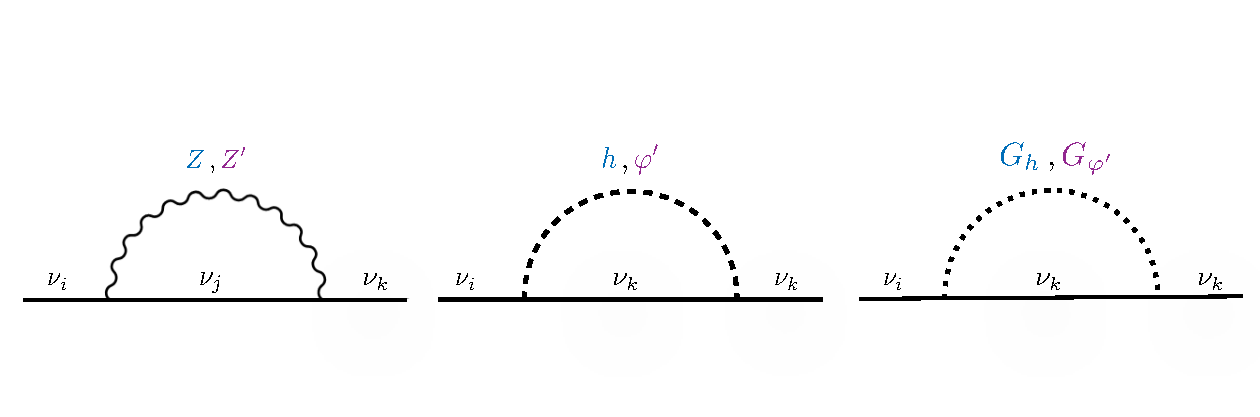
\includegraphics[width=\textwidth]{Loop_masses.pdf}
\caption[]{\label{fig:loops}The three contributions to the neutrino self-energy arising from novel bosons in the theory.}
\end{figure}
%%%%%%%%%%%%%%%%%%%%%%%%%%%%%%%%%%%%%%%%%%%%%%%%%%%%%%%%%%%%%%%

\section{Model set-up} Following~\cite{Ballett:2019pyw}, we add two types of heavy neutral fermions to the SM, namely a dark neutrino $\nu_{D,L} \equiv \nu_{D}$ and a sterile state $N_L \equiv N$. For simplicity, we restrict the discussion to one generation in order to focus on the main features of the model.

We impose a new abelian gauge symmetry $U(1)^\prime$ with associated mediator $X_\mu$ and introduce a neutral complex scalar $\Phi$. No SM fields are charged under $U(1)^\prime$. The scalar $\Phi$ and the fermion $\nu_{D}$ carry the same $U(1)^\prime$ charge, while $N$ remains completely neutral. The gauge-invariant Lagrangian is given by
%
\begin{align} \label{eq:lagrangian}
%
\mathscr{L} =& \mathscr{L}_{\mathrm{SM}} + \left(D_\mu \Phi\right)^\dagger \left(D^\mu \Phi\right) -  V(\Phi,H) \,   \nonumber\\
&  - \frac{1}{4}X^{\mu \nu} X_{\mu \nu} + \overline{N}i\slashed{\partial}N + \overline{\nu_D}i\slashed{D}\nu_D 
 \nonumber\\
&- \left[y^\alpha_\nu (\overline{L_\alpha} \cdot \widetilde{H})N^c + \frac{\mu^\prime}{2}\overline{N}N^c + y_N \overline{N}\nu_D^c\Phi + \text{h.c.}\right],
\end{align}
%
where $X^{\mu\nu} \equiv \partial^\mu X^\nu - \partial^\nu X^\nu$, $D_\mu \equiv \left(\partial_\mu-ig^\prime X_\mu\right)$, $L_\alpha \equiv (\nu_\alpha^T, \ell_\alpha^T)^T$ is the SM leptonic doublet of flavour $\alpha = e, \mu, \tau$ and $\widetilde{H} \equiv i \sigma_2 H^*$ is the charge conjugate of the SM Higgs doublet. In the neutral fermion sector, we have Yukawa couplings $y_\nu^\alpha$ and $y_N$  responsible for $L_\alpha$-$N$ and $\nu_D$-$N$ interactions, respectively, and a Majorana mass $\mu^\prime$ for $N$. The latter term violates by two units any lepton number assignment which leaves 
the Yukawa term $L_\alpha$-$N$ invariant. As such, it plays a crucial role in the generation of light neutrino masses, as we discuss.


We are interested in the case in which both the neutral component of the fields $H$ and $\Phi$ acquire non-vanishing vevs, $v_H$ and $v_\varphi$. They induce mixing between active and heavy fermions, and give a mass to the gauge boson $X_\mu$ and to the real component of the scalar field $\varphi$. We are interested in proposing a model for neutrino masses which is testable in current and future non-collider experiments, and as such we focus on a new physics scale which is below the electroweak one, $v_\varphi < v_H$.  
In addition to the neutrino portal, this model can accommodate a vector portal arising from vector kinetic mixing term and a scalar portal coming from the cross-coupling term $H^\dagger H \Phi^\dagger \Phi$ in the potential~\cite{Ballett:2019pyw}. Kinetic mixing can be reabsorbed in a redefinition of vector fields, leading to a new gauge boson which has vector couplings to the SM fermions proportional to their electric charge. For our neutrino mass generation mechanism, the vector and scalar mixing do not play a relevant role and we set them to zero from here onward, unless otherwise specified. Regarding the vector boson, we refer to it as a $Z^\prime$, independently of kinetic mixing.


%%%%%%%%%%%%%%%%%%%%%%%%%%%%%%%%%%%%%%%%%%%%%%%%%%%%%%%%%%%%%%%%%%%%%%%
\section{Neutrino masses}  
After symmetry breaking, two Dirac mass terms are induced with $m_D \equiv y_\nu^\alpha v_H/\sqrt{2}$ and $\Lambda \equiv y_N v_\varphi/\sqrt{2}$.
For one active neutrino $\nu_\alpha$, $\alpha= e, \mu, \tau$, the mass matrix is given by
%
\begin{align} \label{eq:massmatrix}
\mathscr{L}_{\rm mass} \supset
\frac{1}{2}\left (\begin{matrix} \overline{\nu}_\alpha & \overline{N} &  \overline{\nu_D} \end{matrix} \right )
\left(\begin{matrix} 
     0   &  m_D        & 0 
\\ m_D &  \mu^\prime & \Lambda 
\\   0   &  \Lambda  & 0
\end{matrix}\right)
\left (\begin{matrix} \nu_\alpha^c \\ N^c \\ \nu_D^c \end{matrix} \right) + {\rm h.c.}
\end{align}  
%
Let us emphasize the fact that in our model the zeros in the $\nu_D$-$\nu_D$ and $\nu_\alpha$-$\nu_D$ entries are enforced by the $U(1)^\prime$ symmetry, differently from LSS and ISS models, in which these are generically assumed to be nonzero and small due to the quasi-preservation of lepton number. Here, lepton number violation (LNV) may be large, as the $\mu^\prime$ term breaks it by 2 units. Alternatively, it can be small and technically natural, leading to quasi-degenerate heavy neutrinos, see below. 

After diagonalisation of the mass matrix, the two heavy neutrinos,  $\nu_h$ ($h=4,5$), acquire masses
\[m_{4,5} = \frac{\mu^\prime \mp \sqrt{\mu^{\prime\,2} + 4 (\Lambda^2 + m_D^2) } }{2}.\]
Assuming that $m_D \ll \Lambda$, we focus on two interesting limiting cases. 

The ISS-like scenario is defined by $\Lambda \gg \mu^\prime$: the two heavy neutrinos are nearly degenerate with a mass $\Lambda$ and mass splitting $\mu^\prime$. The relevant mixing parameters are $U_{\alpha 4,5} \sim m_D/\sqrt{2} \Lambda$ and $U_{D4,5} \sim 1/\sqrt{2}$.
The ESS-like case has $\Lambda \ll \mu^\prime$: one neutral lepton remains very heavy, $m_5 \sim \mu^\prime$, and mainly in the completely neutral direction $N$, and the other acquires a small mass via the seesaw mechanism in the hidden sector with $m_4 \sim - \Lambda^2/\mu^\prime$ and $U_{D5} \sim \Lambda/ \mu^\prime$. The mixing with active neutrinos is given by $U_{\alpha 5} \sim m_D/\mu^\prime \ll U_{\alpha 4} \sim m_D/\Lambda$.

The specific form of the mass matrix in Eq.~\ref{eq:massmatrix} implies vanishing light neutrino masses at tree level, as its determinant is zero~\cite{Dev:2012sg,LopezPavon:2012zg}. This feature holds to all orders in the seesaw expansion~\cite{Grimus:2000vj,Adhikari:2010yt,LopezPavon:2012zg}. The light neutrino masses, however, are not protected by any symmetry and arise from radiative corrections (for a review of radiative neutrino mass models see, \eg, Ref.~\cite{Cai:2017jrq}). 



%%%%%%%%%%%%%%%%%%%%%%%%%%%%%%%%%%%%%%%%%%%%%%%%%%
\subsection{Radiative corrections} We now show that our model generically leads to the generation of light neutrino masses at one loop. The calculation of the radiative mass term follows Refs.~\cite{Pilaftsis:1991ug,Kniehl:1996bd} with the addition of the loops with the new boson and scalar particles shown in \reffig{fig:loops}. The self-energy of the Majorana neutrino fields is given by 
%
\begin{equation*}
 \Sigma_{ij}(\slashed{q}) = \slashed{q}P_\text{L}\Sigma^\text{L}_{ij}(\slashed{q}) + \slashed{q}P_\text{R}\Sigma^\text{L*}_{ij}(\slashed{q}) + P_\text{L}\Sigma^\text{M}_{ij}(q^2)+ P_\text{R}\Sigma^{\text{M}*}_{ij}(q^2).
\end{equation*}
%
Using the on-shell renormalization scheme, the renormalized mass matrix for the light neutrinos, massless at tree level, emerges at one-loop and is given by~\cite{Kniehl:1996bd}
%
\[    m_{ij}^\text{one-loop} = \text{Re}\left[ \Sigma^\text{M}_{ij}(0)\right], \quad  i, j <4. \]
%
The self energy can be decomposed as
%
\begin{align}
\Sigma_{ij}^\text{M}(0) = \Sigma^Z_{ij}(0)& + \Sigma^{h}_{ij}(0) + \Sigma^{G_h}_{ij}(0) \,+ \nonumber\\ &\Sigma^{Z^\prime}_{ij}(0) +
\Sigma^{\varphi^\prime}_{ij}(0) + \Sigma^{G_\varphi}_{ij}(0),
\end{align}
where $\Sigma^{Z, h, G_h}$ come from the SM particles, $Z^0$, the Higgs and the associated Goldstone boson, respectively, and $\Sigma^{Z^\prime, \varphi^\prime, G_\phi}$ are the new terms present in our model, mediated by the new gauge boson and new scalar components. From it, we write the $3\times3$ light neutrino mass matrix 
%
\begin{align}\label{eq:masses_general}
 m_{ij} = \frac{1}{4\pi^2}\sum_{k=4}^5 \Big[ & C_{ik} C_{jk} \frac{m_k^3}{m_Z^2}F(m_k^2,m_Z^2,m_h^2)  \,+ 
 \nonumber\\ &D_{ik} D_{jk} \frac{m_k^3}{m_{Z^\prime}^2}F(m_k^2,m_{Z^\prime}^2,m_{\varphi^\prime}^2) \Big], 
\end{align} 
%
where we defined coupling matrices corresponding to the SM and new physics interaction terms assuming $\chi=\lambda_{\Phi H}=0$:
%
\begin{equation} \label{eq:couplings}
C_{ik} \equiv \frac{g}{4c_W}\sum_{\alpha = e}^\tau U_{\alpha i}^*U_{\alpha k}\quad\text{and} \quad D_{ik} \equiv \frac{g^\prime}{2} U^*_{Di} U_{Dk}.
\end{equation}
Equivalent expressions can be found for non-vanishing portal couplings, but considering experimental constraints we find that these do not play a role in the neutrino mass generation. It is possible to show that in general $\sum_{k} m_k C_{ik} C_{jk} =0$ and $\sum_{k} m_k D_{ik} D_{jk} =0$ for any $i,j$. By virtue of the latter property, the loop function can be written as
%
\begin{equation} \label{eq:loop_function}
F(a,b,c) \equiv \frac{3 \, \ln{(a/b)}}{a/b - 1}  + \frac{\ln{(a/c)}}{a/c - 1}.
\end{equation}
%
Turning off the $g^\prime$ gauge coupling, we recover the expression for the Type-I seesaw case~\cite{Pilaftsis:1991ug}:
 \begin{align}  \label{eq:SM_masses}
 m_{ij} = &\frac{\alpha_W}{16\pi}\sum_{\alpha, \beta = e}^{\tau} U_{\alpha i}^\ast U_{\beta j}^\ast  U_{\alpha 5} U_{\beta 5} \frac{m_5}{m_W^2} \times\nonumber\\ & \left( m_5^2 F(m_5^2,m_Z^2,m_h^2) -  m_4^2 F(m_4^2,m_Z^2,m_h^2)\right).
 \end{align}
%
These SM corrections to neutrino masses also arise in the Minimal ISS model~\cite{Dev:2012sg,LopezPavon:2012zg}. In the latter, however, no explanation is provided as to why they dominate neutrino masses. Moreover, if we restrict the discussion to scales well below the electroweak one, $ m_5 \ll 10$~GeV, bounds on the mixing angles severely constrain the parameter space viable to generate the observed values of the masses. 

For a light $Z^\prime$, the second term in Eq.~\ref{eq:masses_general} dominates
%
\begin{align}\label{eq:BSM_masses}
m_{ij} \simeq  &\frac{g^{\prime2}}{16\pi^2} U_{D i}^{*} U_{D j}^{*} \,  U_{D5}^2 \frac{m_5}{m_{Z^\prime}^2} \times\nonumber\\  \quad \quad & \big(m_5^2 F(m_5^2,m_{Z^\prime}^2,m_{\varphi^\prime}^2) - m_4^2 F(m_4^2,m_{Z^\prime}^2,m_{\varphi^\prime}^2)\big)~.
\end{align}
%
We notice that the resulting mass matrix has only one nonzero eigenvalue. This suggests that a typical prediction of our model is a normal ordering mass spectrum, in which $m_3$ is given by this radiative mechanism and $m_2$ has another origin, for example the loops mediated by the SM gauge bosons or by additional particle content. Our simplifying assumption of one generation of hidden fermions is by no means necessary and more generations of new fermions are possible, leading to a much richer structure for the light neutrino mass matrix. The additional $\mu^\prime$ terms would not be constrained and could be at different scales, while the $\Lambda$ terms arise from the $U(1)^\prime$ breaking and are therefore constrained to be at/below $v_\varphi$. Therefore, the full model could present a combination of relatively light Majorana $\nu_h$, mainly in dark direction, some very heavy nearly-neutral neutrinos and pseudo-Dirac pairs at intermediate scales. A discussion of this extension is beyond our scope, but we note that it has interesting consequences for both the heavy and light neutrino mass spectra and mixing structure.

Working in a single family case, we derive expressions for Eq.~\ref{eq:BSM_masses} in the seesaw limit for both the ISS and ESS-like scenarios. %%%%%%%%%%%%%%%%%%%%%%%%%%%%%%%%%%%%%%%%%%%%%%%%%%%%
% ISS
In the ISS-like regime and assuming $m_{Z^\prime}, m_{\varphi^\prime} \ll \, \Lambda$, \refeq{eq:BSM_masses} simplifies to
%
\begin{align} \label{eq:ISSlimit_1}
m_3 \simeq& \frac{g^{\prime 2}}{8\pi^2} \frac{m_D^2}{m_{Z^\prime}^2} \mu^\prime  \left( {3 \ln{\frac{m_{Z^\prime}^2}{\Lambda^2}} + \ln{\frac{m_{\varphi^\prime}^2}{\Lambda^2}} - 4 }\right),
\end{align}
%
while for $m_{Z^\prime}, m_{\varphi^\prime} \gg \, \Lambda$ it reduces to 
%
\begin{align} \label{eq:ISSlimit_2}
m_3 \simeq& \frac{g^{\prime 2}}{16\pi^2} \frac{m_D^2}{\Lambda^2} \mu^\prime \left( 3 + \frac{m_{\varphi^\prime}^2}{m_{Z^\prime}^2} \right).
\end{align}
%
As it can be expected, neutrino masses are controlled by the LNV parameter $\mu^\prime$ and are enhanced with respect to the SM contribution by a factor of $(m_Z/m_{Z^\prime})^2$ in the former, or $(m_Z/\Lambda)^2$ in the latter case. 

For the ESS-like regime, taking $m_{Z^\prime}, m_{\varphi^\prime} \ll \mu^\prime$, the light neutrino mass is approximately
%
\begin{align} \label{eq:ESSlimit_1}
m_3 \simeq& \frac{g^{\prime \,2}}{16\pi^2} \frac{m_D^2}{\Lambda^2 + m_D^2} \frac{\Lambda^2}{m_{Z^\prime}^2} \mu^\prime  \left( {3 \ln{\frac{m_{Z^\prime}^2}{ \mu^{\prime 2} }} + \ln{\frac{m_{\varphi^\prime}^2}{ \mu^{\prime 2} }}}\right),
\end{align}
%
while for $m_{Z^\prime}, m_{\varphi^\prime} \gg \mu^\prime$, it is
%
\begin{align} \label{eq:ESSlimit_2}
m_3 \simeq& \frac{g^{\prime 2}}{8\pi^2} \frac{m_D^2}{\Lambda^2+m_D^2} \frac{\Lambda^2}{\mu^\prime}  \left( {3 \ln{\frac{m_{Z^\prime}^2}{\Lambda^2}} + \ln{\frac{m_{\varphi^\prime}^2}{\Lambda^2}} - 4 }\right).
\end{align}
%
In this case, the light neutrino masses are controlled mainly by $\nu_5$, and the intermediate state $\nu_4$ can be much lighter. 
%
\begin{figure*}[t]
    \centering
    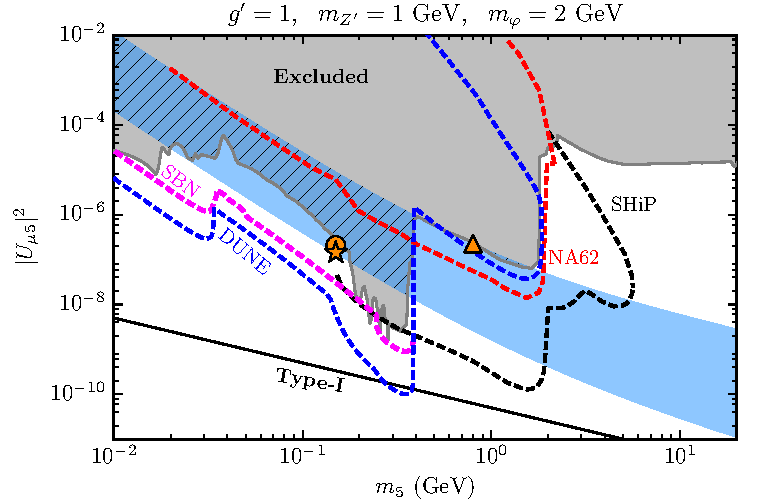
\includegraphics[width=0.49\textwidth]{paper_plot_nu5_highmz.pdf}
    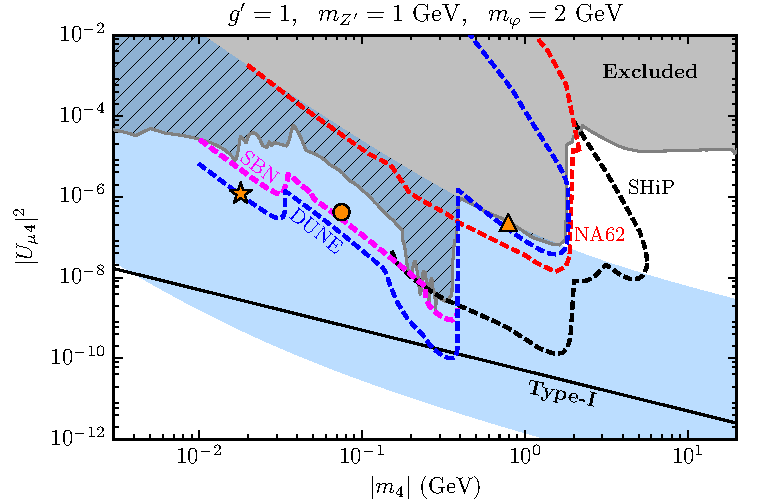
\includegraphics[width=0.49\textwidth]{paper_plot_nu4.pdf}
    \caption[Region of interest for neutrino mass generation in our model.]{The region of interest for neutrino mass generation in our model in the parameter space of the $\nu_5$ (left) and $\nu_4$ (right) mass states. We require $m_3 = \sqrt{\Delta m^2_{\rm atm}}$ and vary $1\%<m_4/m_5<99\%$. Our BPs are $\bigtriangleup$) $m_5 = 800$ MeV, $m_4/m_5 =99\%$, ${\circ}$) $m_5 = 150$ MeV, $m_4/m_5 =50\%$ and $\star$) $m_5 = 150$ MeV, $m_4/m_5 =12\%$. All bounds and projections displayed assume $\chi=\lambda_{\Phi H}=0$. The dashed black line shows the equivalent Type-I seesaw contribution to the light neutrino mass.\label{fig:mass_constraints}}
\end{figure*}

%%%%%%%%%%%%%%%%%%%%%%%%%%%%%%%%%%%%%%%%%%%%%%%%%%%%%%%%%%%%%%%%%%%%%%%
\section{Searching for the origin of neutrino masses} \label{sec:pure_nu_mixing}

In what follows, we discuss the experimental reach to the heavy neutrinos responsible for neutrino mass generation in our model. Since the vector and scalar portals do not contribute significantly to neutrino masses, we first restrict the study to the case $\chi=\lambda_{\Phi H}=0$. For the sake of simplicity and concreteness, we work with a single generation of light neutrinos and focus on the mixing with the muon neutrino. We emphasise that our model predicts
%
\begin{equation}
    \frac{m_4}{m_5} = - \frac{U_{\alpha 5}^2}{U_{\alpha 4}^2},
\end{equation}
%
implying that both heavy neutrinos should be searched for.
%
For a real mixing matrix one can write $\sum_i^3 U_{D i}^{2} \sim U_{\mu 4}^{2}$ and $U_{D 5}^{2} \sim 1$ for small $U_{\mu 4}$. Using these relations and \refeq{eq:masses_general}, we plot the region of interest for neutrino mass generation in \reffig{fig:mass_constraints}. We require $m_3 = 
\sqrt{\Delta m^2_{\text{atm}}} \sim 0.05~\text{eV}$ and vary $m_4/m_5$ from $1\%$ (ESS-like) to $99\%$ (ISS-like). For the hidden sector parameters, we fix $m_{Z^\prime}=1$~GeV, $m_{\varphi^\prime} = 2$ GeV and $g^\prime = 1$. By decreasing (increasing) the mass of the $Z^\prime$, it is possible to shift the band to smaller (larger) values of the mixing angles, although for values smaller than a few hundred MeV, the neutrino masses have a very mild dependence on $m_{Z^\prime}$ (Eqs.~\ref{eq:ISSlimit_2} and~\ref{eq:ESSlimit_2}). Increasing $m_4/m_5$ to values closer to $100\%$ (\ie\,, decreasing $\mu^\prime$ below $m_5/100$) shifts the top of the band to larger values of mixing angle and asymptotically recovers lepton number as a symmetry. Although this possibility appears excluded for $m_{Z^\prime} = 1$ GeV, it can be achieved by lowering the mass of the mediator particles. For instance, for $m_{Z^\prime} = m_{\varphi^\prime}/2 = 100$ MeV and $m_5 < 100$ MeV, we find that values as small as $\mu^\prime \gtrsim 10^{-3} m_5$ are not covered by the grey region in \reffig{fig:mass_constraints}.
Values of $m_4/m_5 < 1\%$ have no effect in the parameter space of $\nu_5$, since in that limit the $\nu_5$ state (mostly in the $N$ direction) dominates the loop contribution.

The region labelled as excluded in \reffig{fig:mass_constraints} is composed of bounds from peak searches~\cite{
%KEK
Yamazaki:1984sj,
%NA48/2
Artamonov:2014urb,
%NA62
CERNNA48/2:2016tdo}, beam dump \cite{
%PS-191
Bernardi:1985ny,
%CHARM
Bergsma:1983rt,
%NA3
Badier:1986xz,
%NuTeV
Vaitaitis:1999wq, 
%BEBC
CooperSarkar:1985nh, 
%NOMAD
Astier:2001ck} 
%
and collider experiments~\cite{
Abreu:1996pa,%DELPHI
Akrawy:1990zq,%OPAL
Sirunyan:2018mtv% CMS 2018
}. Current and future neutrino experiments can also cover a large region of parameter space with $m_h \lesssim 2$ GeV. For instance, we show the sensitivity of the Short-Baseline Neutrino program (SBN)~\cite{Ballett:2016opr} and of the Deep Underground Neutrino Experiment (DUNE) near detector~\cite{Ballett:2018fah,Ballett:2019bgd} to heavy neutrinos in decay-in-flight searches. We also show the reach of the NA62 Kaon factory operating in beam dump mode~\cite{Drewes:2018irr}, and the dedicated beam dump experiment Search for Hidden Particles (SHiP)~\cite{Bonivento:2013jag,Alekhin:2015byh}, which will cover a much larger region of parameter space from $400$ MeV to $\lesssim6$ GeV. All bounds and sensitivities shown do not take into account the new invisible decays of the heavy neutrinos. Searches that rely on the visible decay products of the heavy neutrinos need to be revisited if the $\nu_h$ can decay invisibly or if new channels mediated by the vector (and/or scalar) portal dominate. In particular, faster decays of $\nu_h$ can shift decay-in-flight bounds to lower values of mixing angles, as discussed in detail in Ref.~\cite{Ballett:2016opr}. Peak searches apply as shown provided $\nu_h$ does not decay immediately via neutral-current channels with visible charged particles.

Let us first consider the case of subdominant vector and scalar portals. Compared to the ``standard" sterile neutrino case, in which $\nu_h$ have only SM interactions suppressed by neutrino mixing, the new neutral-current interaction can enhance the $\nu_h$ decays into light and heavy neutrinos. A comprehensive analysis is beyond the scope of this article and we focus on three benchmark points (BP) shown in \reffig{fig:mass_constraints} to exemplify the most characteristic properties. The BP represented as a triangle ($\bigtriangleup$) corresponds to $m_5 = 800$ MeV and $m_4/m_5 = 99\%$. In this case, the two heavy states are very degenerate in mass and decay like a ``standard" sterile neutrino via $|U_{\mu 4}|^2$-suppressed SM charge- and neutral-current interactions. The channel $\nu_5 \to \nu_4 \nu_\alpha \overline{\nu}_\alpha$ via the $Z^\prime$ is phase space suppressed and becomes relevant only for larger mass splittings. The invisible $\nu_4$ decay mediated by the $Z^\prime$ is subdominant as it scales as $|U_{\mu 4}|^6$ and becomes important only for larger values of the mixing angles.

For the next BPs we fix $m_5 = 150$ MeV. If we take $m_4/m_5 = 50\%$, as we do for the BP represented by the circle ($\circ$), $\nu_5$ will predominantly decay to $\nu_4 \nu_\alpha \overline{\nu}_\alpha$ due to the $Z^\prime$ contribution (provided $|U_{\mu 5}|^2\gtrsim \left( m_{Z^\prime}/m_{Z} \right)^4$). Consequently, the best candidate for detection is the $\nu_4$ via the SM weak decays $\nu_4 \to \nu_\alpha e^+e^-$. The values of the mixing angles for this BP, $|U_{\mu 4}|^2 \sim 3\times 10^{-7}$ and $|U_{\mu 5}|^2 \sim 10^{-7}$, are within reach of the SBN and DUNE experiments. 
For a larger mass hierarchy, e.g. $m_4/m_5 = 12\%$, see star BP ($\star$), the $Z^\prime$ mediated decay $\nu_5 \to \nu_4 \overline{\nu_4} \nu_4$ dominates, inducing a large $\nu_4$ population in addition to the states already produced in the beam. The intermediate state $\nu_4$ can further decay as in the previous case into $\nu_4 \to \nu_\alpha e^+e^-$. For the mixing angles we are considering, $|U_{\mu 4}|^2 \sim 10^{-6}$ and $|U_{\mu 5}|^2 \sim 10^{-7}$, DUNE will be able to test this BP. Similar considerations apply to the case where $m_5 > m_4 + m_{Z^\prime}$, where now the $Z^\prime$ can be produced on-shell in the $\nu_5$ decay. The behaviour of $\nu_4$ is as discussed above. If $ m_{Z^\prime} < m_4$, then both heavy neutrinos predominantly decay into neutrinos and the $Z^\prime$, which presents a challenge for detection as it produces mainly light neutrinos.

Experimental detection of the $Z^\prime$ and $\varphi^\prime$ particles in the absence of kinetic and scalar mixing is also daunting. Nevertheless, they can be searched for in the kinematics of charged particles from meson decays~\cite{Laha:2013xua,Bakhti:2017jhm}. Another strategy is to search for the neutrino byproducts of the decay of a $Z^\prime$ produced at accelerator neutrino facilities~\cite{Bakhti:2018avv}. 

If the vector (and scalar) portals are non-negligible, the phenomenology could be significantly richer, as discussed in \cite{Ballett:2019pyw}. In particular, $Z^\prime$-mediated decays into $\nu_\alpha e^+ e^-$, and $\nu_\alpha \mu^+ \mu^-$ if kinematically allowed, could dominate even for tiny values of $\chi^2$. For instance, for the circle BP, $\chi^2 $ as low as $10^{-8}$ would make the above decays the main channels. Pseudo-scalar final states are suppressed due to the vector nature of the $Z^\prime$. The scalar portal is expected to give subdominant contributions due to the small Higgs-electron Yukawa coupling, although decay chains with intermediate $\nu_4$ states may become relevant. Finally, cosmological bounds on heavy neutrino in the 10 MeV -- GeV scale may be weakened as they would decay well before Big Bang Nucleosynthesis~\cite{Dolgov:2000jw} (see also the discussion in Ref.~\cite{Hannestad:2013ana,Dasgupta:2013zpn,Mirizzi:2014ama,Chu:2015ipa,Cherry:2016jol,Chu:2018gxk,Song:2018zyl})%The BR would have a very different structure compared to the standard neutrino and vector portals. By looking for the decay channels, one would be able to, at least partially, disentangle the neutrino, vector and scalar contributions.

We have focused on the mixing with muon neutrinos as these provide one of the most sensitive avenue to test the model. In the electron sector, direct bounds on the active-heavy mixing are similar, with peak searches from $\pi^\pm$ decay being most relevant below $\approx 100$ MeV. For cases with large LNV, heavy neutrinos can dominate neutrinoless double beta decay~\cite{LopezPavon:2012zg}, and this sets the strongest constraints in the parameter space. The tau sector is relatively poorly constrained, so greater freedom exists if such entries are relevant for neutrino mass generation. 


